\begin{frame}{あらためてメッシュ要素について復習}
  \begin{table}[hbtp]
      \caption{3次元構造解析で使われる主なメッシュ要素(一部)<参考文献\cite{handbook}>}
      \vspace{-5mm}
      \begin{tabular}{|r|c|c|c|} % 表は項目名を右寄せ、データを中寄せ
          \hline
          名称       & 4面体2次要素 & 6面体1次要素 & 4面体1次要素 \\
          \hline
          接点配置   & 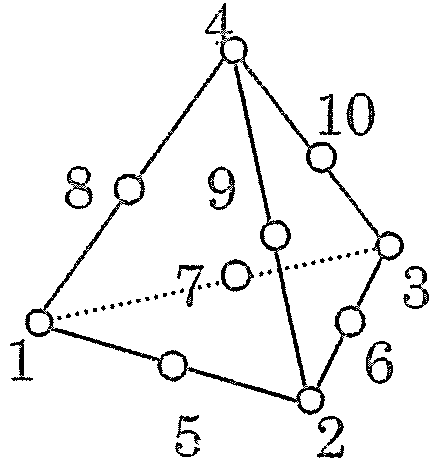
\includegraphics[keepaspectratio]{work/images/tet10.png}
                     & 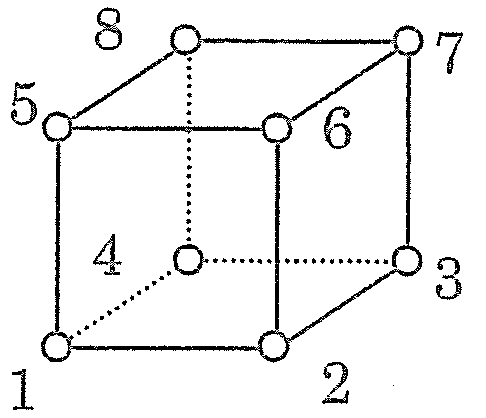
\includegraphics[keepaspectratio]{work/images/hex8.png} 
                     & 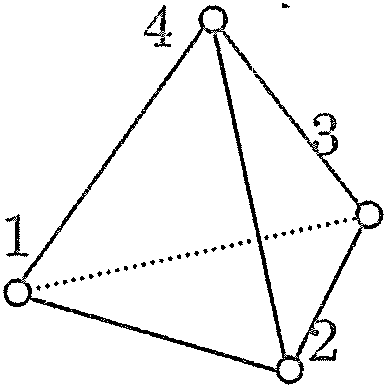
\includegraphics[keepaspectratio]{work/images/tet4.png}  \\
          \hline
          メリット   & 任意の形状で切れる & 見た目が美しい & 無 \\
          \hline
          デメリット & 多少見た目が悪い   & 形状に人間の介入が必要 & 硬い \\
          \hline
          評価       &   〇               & ◎              & × \\
          \hline
    \end{tabular}
  \end{table}
  %
  ※ 他に5面体1次要素(6面体1次要素の面が一つ縮退したもの)もある
  %
  \only<2>{
    % TiKZを使った図形の描画 使用禁止札
    \begin{textblock*}{30pt}(385pt,105pt)
      \begin{tikzpicture}
         \node[rectangle,fill=cud_yellow,text width=0.5cm,text centered,rounded corners,minimum height=0.5cm](s) at (1cm,1cm) { \scriptsize 使用禁止};
      \end{tikzpicture}
    \end{textblock*}
  }
\end{frame}
